\documentclass[10pt]{article}

\usepackage[usenames,dvipsnames]{pstricks}
\usepackage{epsfig}
%\usepackage{pst-grad} % For gradients
%\usepackage{pst-plot} % For axes


\usepackage{graphicx, subFigure}

\usepackage{amsmath} % for the argmin
\usepackage{amsfonts}


\newcommand{\argmax}[1]{\underset{#1}{\operatorname{argmax}}}
\newcommand{\argmin}[1]{\underset{#1}{\operatorname{arg\ min}}}
\setlength{\parindent}{0in}
\newcommand{\code}[1]{\texttt{#1}}

\newcommand{\fig}[3]{
	\begin{figure}[!ht]
	\centering
	\includegraphics[scale=#3]{img/#1}
	%\includegraphics[width=420px]{img/#1}
	\caption{#2}
	\label{fig:#1}
	\end{figure}
}
\newcommand{\fignocaption}[3]{
	\begin{figure}[!ht]
	\centering
	\includegraphics[scale=#3]{img/#1}
	\label{fig:#1}
	\end{figure}
}

\newcommand{\figw}[3]{
	\begin{figure}[!ht]
	\centering
	\includegraphics[width=#3]{img/#1}
	\caption{#2}
	\label{fig:#1}
	\end{figure}
}

\newcommand{\figs}[6]{
	\begin{figure}[!ht]
	\centering
	\subfigure[#5]{
		\includegraphics[width=14cm]{img/#2}
		\label{fig:#2}
	}
	\subfigure[#6]{
		\includegraphics[width=14cm]{img/#3}
		\label{fig:#3}
	}
	\caption{#4}
	\label{fig:#1}
	\end{figure}
}
\newcommand{\figsSmall}[6]{
	\begin{figure}[!ht]
	\centering
	\subfigure[#5]{
		% width=14cm
		\includegraphics[width=5cm]{img/#2}
		\label{fig:#2}
	}
	\subfigure[#6]{
		% width=14cm
		\includegraphics[width=5cm]{img/#3}
		\label{fig:#3}
	}
	\caption{#4}
	\label{fig:#1}
	\end{figure}
}


% TODO
% put this in one of the chapters before this chapter:
% an intro which answers the question:
% detail of the problem, why is this such a interesting problem
% what did others and how is my work related?

\title{\sc Improve 3D models from 2D images}

\author{T. Kostelijk\\mailtjerk@gmail.com}

\begin{document}
\maketitle


% LaTeXDraw 
% op uva compu compilen?


\section{Comments on this thesis}
Dear Isaac,

This in an update of my thesis chapter. I incorporated most of the feedback except for\\
-the test on different datasets\\
(the dataset is not ready yet)\\
-references\\
-large introduction\\
I expanded the introduction a bit more then my previous version but I think you want more background
information. I do this in a few chapters earlier which is not included in this document.\\
I processed a lot of small changes and the two big changes are:\\
I updated the way line segments are associated with building parts and illustrated it with Figure 10.\\
I wrote a new subsection about alternative roof-types.\\
Thanks in advance for reading my thesis chapter and giving me usefull feedback.

 
\section{Improving the 3D building}
\subsection{Introduction}
%chain
In the previous chapter we extracted the building contour with the skyline
detector. The output was a set of 2D points and we collected this set for every
view of the building.  The aim of this chapter is to use this set of points to
improve the basic 3D model. 

The point cloud from the skyline detector included a lot of noise caused mostly
by occluding objects like tree's. How do we detect those outliers?
And if we have an outlier free point cloud how can we use this information to
improve the 3D model? How can a point be associated to a specific part of the
building and finally improve the 3D model? 
These questions are addressed in this chapter.

%solution
We present a stepwise solution. First \emph{Openstreetmap} is used to generate
a basic 3D model of a building. Secondly the set of points returned by the
skyline detector is transfered to a set of lines. Then each line segment is
assigned to a wall of the building. After this the lines are projected to these
assigned walls in the 3D model. 
These projections are used to estimate the new heights of the building walls.
The 3D model is then improved by updating the walls according these heights. \\
We will now elaborate on the steps.

\subsection{Generating the 3D model}
% --------------------------------------

\emph{openstreetmap} gives us a photo of the
building.  The heights of the walls are unknown because a top view of the
building is used.  
From this top view image a basic 3D model with infinite
height walls is generated.\\





% TODO example image openstreetmap
The generated 3D model is inspired by \emph{Openstreetmap}.  Openstreetmap is
a freely accessible 2D map generated by users all over the world. It contains
information about streets, building contours, building functions, museums, etc.
We are interested in the building contours.  We take a snapshot of one
particular area and extract the buildings information.  This is a set of
ordered points that can be connected.  Each point corresponds to a corner of
the building and these points can be linked to walls.  The map is in 2D and
therefore contains no information about the height of each wall.  Also
information regarding the rooftype or the number of floors is not present.

We generate a 3D model by using the 2D buildingcontour of \emph{openstreetmap}
and estimate the wall heights by hand.  This is only for illustration purposes,
the algorithm actually works with infinite planes which are spanned by the
these walls. An example of the 3D model can be seen in Figure 3.
% TODO Fig nr


% TODO
% part of intro?:
% And if we know which data belongs to the building contour we could use the developed projection techniques from section %TODO
% to obtain parts of the building contour.
% The next question arises is, given this building contour parts, how do we
% improve the 3D model in a clean way?

%before we take these next steps we take one step back and go to the 2d images.
	%we saw that the skyline detector outputs a binary image where a white pixel is considered as highly from the skyline and therefor the building contour.
	%TODO


% why not ransac?
\subsection{Extracting line segments}
% Let us first define the input of the algorithm:
% \begin{itemize}
% 	\item a set of calibrated binary 2D images where white indicates a skyline pixel which has a high probability of being the building contour
% 	%TODO explain calibrated somewhere eerder in het report
% 	\item a rough 3D model extracted from an open street view database
% \end{itemize}
%
% The output will be an updated 3D model, this output is developed in several steps:\\
% First some operation are done in 2D, the individual skyline pixels are grouped
% into line segments using an approach called the Hough transform. In the next
% step every line is heuristicly associated to (and projected on) a specific wall
% in 3D. The third step is to combine the projected line segments, which produces
% and estimate of the height of each building wall. In the last step these heights
% are used to improve the walls of the rough 3D model.

%why fit lines on 2d and not in 3d
%cheaper easier?

	%TODO CHANINGI
	% In the introduction we talked about the 
	% the sake of outlier removal for the Skyline detector.

	To remove the outliers the process is reversed: we detect the
	inliers and consider the remainder as outliers. But we first have to define an inlier.\\
	Lets take the contour of an average building, this is mostly formed by
	straight lines. We use this fact to simplify our problem:\\
	\emph{Flat roof assumption}\\
	\emph{We assume each building has a flat roof, implicating that each building-wall
	has a straight upper contour}

	% TODO example images
	If a set of skyline pixels lie on the same line, they form a straight line
	and therefor have a large probability to present a part of the building contour.
	These skyline pixels, that form a straight line, are therefor considered as our
	inliers.\\ 
	If we have a method that extracts straight line segments, we can use these
	line segments to find parts of the building contour and finally use this to improve the 3D
	model. Next is explained how these straight line segments are extracted.
	

\subsubsection{Hough transform}
	A widely used method for extracting line segments is the Hough transform
	(invented by P. Hough).  We regard this as a suitable method because it is
	used a lot for this kind of problems. This is probably because it is unique
	in its low complexity (compared to other (iterative) methods like
	\emph{RANSAC}).
	%TODO reference
	%TODO aan alle eind alinea \\ zetten
	We will explain this method briefly.\\
	In the Hough transform, a main idea is to consider the characteristics of a
	straight line not as its image points $(x1, y1)$, $(x2, y2)$, etc., but in
	terms of the parameters of the straight line formula $y = mx + b$. i.e., the
	slope parameter $m$ and the intercept parameter $b$.\\
	The input of a Hough transform is a binary image, in our case the output of 
	the skyline detector (chapter TODO).\\
	If a pixel is classified as a skyline pixel (a pixel that lies on the
	skyline according the skyline detector), the Hough transform increases
	a vote value for every valid line ($m$,$b$ pair) that crosses this
	particular pixel.  Lines ($m$, $b$ pairs) that receive a large amount of votes
	contain a large amount of skyline pixels.\\
	Because the algorithm detects straight lines containing only skyline pixels it is
	most likely that it returns parts of the skyline and therefor the building contour. \\
	The Hough transform is implemented in \emph{Matlab} and has some useful extra functions.\\
	The algorithm can optionally return the start- and endpoint of the found lines 
	which is very useful as it helps to associate which part of the building is described by the line.
	Furthermore it has the parameter \emph{FillGab} that specifies the distance
	between two line segments associated with the same $m$,$b$ pair. When the
	distance between the line segments is less then a specific value specified, it merges
	the line segments into a single line segment. In our application this
	parameter is of particular interest when we want to merge lines that are
	interrupted by for example an occluding tree.\\
	%TODO ga ik daar nog iets over zeggen?
	%Because of occlusion the Houghlines could return two separate line segments
	%which is originally one line which is %onderbbbbbbbroken.  \\
	Results of the Hough transform on the 2D output of the skyline detector are
	displayed and evaluated in the Result section.



\subsection{Associating line segments with building parts}
% 	method below is very nice but it is outperformed by my ultragenius other
% 	method, so I could use it in the thesis but only as different test
% 	methods
%
% 	It would be straightforward to use the method of chapter %TODO
% 	Instead of a skyline pixel we could take the line segments endpoints and project it onto the building walls. The wall with the shortest distance will be assigned to the line segment.
% 
% 	%And to update the specific wall we first need to know with a high probability of being correct which wall the line segment presents
% 	But this method introduces a problem: some of the line segments have endpoints that lie at the corner of the building. These line segments could easily be associated with the neighboring wall. Because the 3D model is a rough estimate this could lead to bad results.
% 	In the corner case it is not clear to which wall the line segment belongs because both endpoints do not agree on the same wall. To solve this problem some heuristic methods are developed and tested. The following heuristic is both simple and effective.
% 	The heuristic uses the importance of the middle point of the line segment. This middle point has a low change of being on a building corner and the on average biggest change of being on the wall we are looking for.
% 	Therefor we discard the endpoints and use the middle point the endpoints to determine the right wall.
% 	As in the previous section %TODO
% 	this middle point is intersected with all planes spanned by the walls. The line segment is stored to the wall with the shortest distance.
% 	The output of this part of the algorithm is for every wall a bunch of associated line segments originated from different views.
% 
% 	%TODO example image
%TODO name different methods and put in table and test
% Some different methods
% method 1:
% take endpoints and project, con: endpoints don't agree
% see above tekst
% method 2:
% middle point
% method 3: 
% overlap

	% intro
	\subsubsection{Introduction}
	The Hough transform of the previous section returned a set of 2D line
	segments.  If we could find a way to associate parts of the building with
	the 2D line segments, we can use this to improve our basic 3D model.
	This section explains how we associate the line segments with the best 
	matching parts of the building. \\

	First the problem is analyzed and a few assumption are made.  Then some
	heuristics are defined and finally the developed method is explained.
	\subsubsection{Assumptions}
	% intro of assumptions
	We treat the parts of the building as individual walls and associate each
	line segment with a wall of the building that is most likely responsible for
	that line segment. 

	\emph{Unique wall assumption}:\\
	%motivation, straight lines, skyline detector
	\emph{We assume that the output of the Hough transform are line segments that
	each represent the upper side of the contour of a single wall of the building}

	%We assume that the output of the Hough transform, the 2D line segments this set
	%represents (parts of) the building contour. To be more precise we assume
	%that every line segment in the set represents (a part of) the upper side of
	%a specific wall of the building. 


	If a line segment is assumed to represent a single wall then the
	projection to that wall should have a large line-wall overlap. To be more
	precise, lets define $l$ in $\mathbb{R}2$ as a line segment that is generated by the Hough
	transform.  If we project $l$ to the plane spanned by a certain wall $W$, we
	get a line $l_{proj_W}$ in $\mathbb{R}3$.  As we assumed, $l$ comes from the 
	contour of wall $w$. It's easy to see that $l_{proj_W}$
	should have a large overlap with $W$, and also should have a small overlap with
	the other walls.
	%see Figure%TODO. create two Figure's (2d and 3d) with a single houghline
	%(projected)
	
	\emph{Largest line-wall overlap assumption}:\\
	\emph{A line segment is originated from the wall with the largest overlap
	with the projected line segment.}\\

	Now we have defined the assumptions we explain the algorithm.

	\subsubsection{Algorithm}
	The algorithm can be described broadly as follows:\\
	A line segment is projected to all walls and the amount of line-wall overlap is
	calculated. The wall with the largest overlap with the specific line
segment is classified as the most likely wall for that line segment.
	Next the line segments are projected to their most likely wall, the
	algorithm outputs this set of lines in $\mathbb{R}3$. 
	
	%\paragraph{Line wall overlap type}
	This line-wall overlap is calculated in different steps.
	First different types of overlap are explained. After the algorithm
	determines the \emph{overlap type}, the overlap amount is determined and
	normalized.

	$l_{proj_W}$ can overlap $W$ in four different scenarios, this is explained
	in Figure 10. The wall $W$ is spanned by $abcd$, and $l_{proj_W}$ is spanned
	by $vw$.
	

	% fig only works with pdflatex, hmmz, but then fig nr's don't work
	\begin{figure}[!ht]
	\centering
	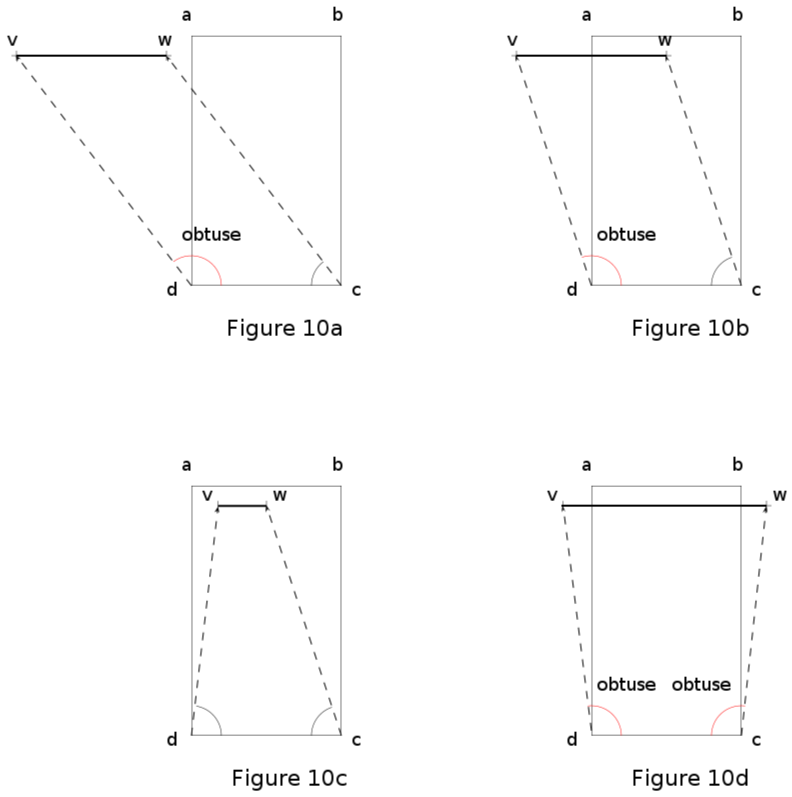
\includegraphics[width=12cm]{img/overlaytypes.png}
	\end{figure}
		

% captions of the Figure
%		1) no overlap (see fig 10a)\\
%		2) partial overlap (fig 10b)\\
%		3) full overlap ($l_{proj_w}$ is included in $w$)(fig 10c)\\
%		4) full overlap ($l_{proj_w}$ overextends $w$) (fig 10d)\\

	The type of overlap is defined by exposing the endpoints of the line
	segments to an \emph{in polygon} test where the polygon represents a 
	wall of the building.
	%TODO REF MATLAB?
	%we use the Matlab build in polygon as in section (%TODO)

	The table below represents the types of overlap with the corresponding number of points
	that pass the \emph{in polygon} test and their possible line-wall overlap
	value.\\ 

	\begin{tabular}{|l||c|c|}
	\hline
	Type of line-wall overlap 			&	points in polygon 			& line-wall overlap \\
	\hline
	\hline
	no overlap					&	0					& 0		\\
	\hline
	partial overlap 				&	1					& [0..1]	\\
	\hline
	full line-wall overlap (included)		&	2					& 1		\\
	\hline
	full line-wall overlap (overextended)		&  	0					& 1 		\\
	\hline
	\end{tabular}

	\paragraph{No overlap}
	If the point in polygon test returns 0, the line-wall overlap calculation
	is skipped and 0 is returned. The remaining overlap types, partial and full,
	are treated individually:\\

	% TODO latex draw
	% latex draw, show cut off line segments (different color)
	% extra dikke vector over de lijn DC
	% duidelijke pijl aan het eind van stippellijn
	% alpha of beta teken en daar naar verwijzen ipv vectors benoemen
	% TODO in Figure overlap ratio percentages drawwen
	% TODO Controleren of het paragraph of susubsections moeten zijn
	% in code \lprojw ipv v,w  zo ook met angles
	% dikke W in abcd vlak


	\paragraph{Partial overlap}
	Lets first consider the partial overlap type (Figure 10b), the \emph{in polygon} test
	returned 1, that means that one of the line segments endpoint lies inside
	and one lies outside the wall.\\
	To calculate the amount of line-wall overlap, the line segment is cropped to the
	part that overlaps the wall and the length is measured.\\
	The cropped line has two coordinates, first of course the point that passed
	the \emph{in polygon} test and secondly the intersection of the line
	segment with one of the vertical wall sides.\\
	(Note that because we assume the walls to be of infinite height, the 
	partial overlapping line segment always intersects one of the
	vertical wall sides.)\\
	To determine which of the two vertical wall sides ($da$ or $cb$ from Figure 10b)
	 is crossed, we determine on which side the point that didn't lie in the polygon (v) lies.
	This is done by an angle comparison (as in section TODO).\\
	First, two groups of two vectors are defined: $dv$, $dc$ and $cw$, $cd$ (see Figure 10b).
	We measure the angles between the vectors and call them $\angle d$, and
	$\angle c$. 
	Because one of the line segment endpoints lies outside
	the wall $\angle d$ or $\angle c$ is obtuse, in this case $\angle d$ is obtuse.
	(Note that this only holds under the assumption that all wall sides are orthogonal)\\
	To be more precise: 
	\begin{itemize}
	\item if $\angle d$ is obtuse, the left vertical wall side $da$, is
	crossed. \\
	\item If $\angle c$ is obtuse, the right vertical wall side $cb$, is
	crossed. \\
	\end{itemize}
	(The angles are acute or obtuse if the dot product of the vectors involved
	are respectively positive or negative. The advantage of this method is that
	it's simple and has low computational costs.)
	The amount of line-wall overlap is easy calculated by cutting of the
	point where $l$ intersects the determined vertical wall side ($da$ or
	$cb$) and measuring its remaining length.

	\paragraph{Full or no overlap}
	Now lets consider the overlap types where the \emph{in polygon} test
	returned 0.
	As you can see in Figure 10a and 10d this resulted in either full- or no overlap.
	Again we analyze the vector angles to determine the remaining overlap-type.
	If only one of the angles is obtuse, Figure 10a, with no points in the polygon 
	then the whole line segment lies outside the wall. An overlap value of zero
	is returned.\\
	Otherwise, if both angles $\angle d$ and $\angle c$ are obtuse or acute (Figure 10d),
	both endpoints lie on a different side of the wall, and cross the wall somewhere in
	between. Full overlap is concluded here. \\
	The amount of overlap is now calculated by measuring the length
	of the line segment which is cut down by his intersections with $da$ and
	$cb$. In this case this is the same as line $dc$, but its easy to see that
	this is not the case when the $vw$ is skew.\\
	
	Finally the line-wall overlap is normalized by the line segments length:\\
	%TODO different math mode
	$\alpha_l = \frac{lwo}{|l|}$\\
	Where $\alpha_l$ is the normalized line-wall overlap, $lwo$ is the unnormalized
	amount of line-wall overlap, and ($|l|$) is the total length of the line
	segment.\\
	The intuition behind this is that line segments that are likely to
	present a wall not only have a large overlap but also have a small part
	that has no overlap. By calculating the relative overlap, both amount of overlap
	and -missing overlap is taken into account.\\
	The maximum of the normalized line-wall overlap is used to associate a
	line segment with its most likely wall.
	%TODO formula?
	\emph{should I place a formula here? and if yes how do I denote this
	mathematically legal/correct}\\
	To summarize, the overlap type is defined by calculating the numbers of in
	polygon points and measuring some angles. Next the line segment is cut off
	depending on the overlap type and the line is normalized. A search for the
	maximum normalized line-wall overlap is used to determine the correct line-wall
	association.\\

	%TODO
	% example image where I project a line to every wall of the building
	% a table of wall overlap value's sorted on largeness
	% bedenken: hoezo wint niet altijd de achterste wall omdat er dan full overlap
	% is??



	% TODO:
	% make schema with 3 methods, and in one regel the summary of its technique
	
	% test with different techniques
	% make different dataset
	% hand anotated (pleonastisch zeg hehe) for ground truth
	% 1) project endpoints (and sometimes end up not agreeing wall)
	% 2) use midpoint of line
	% 3) use tjs algo (line wall overlap)

\subsubsection{Wall height estimation}
  	In the previous section we associated the line segments with their most
	likely wall. In this section this information is used to estimate the height of the
	wall which is finally used to update the 3D model in the next section.
	\\
	Now all line segments are associated with a certain wall we re-project the
	line segment from the different views on their associated wall. The
	re-projection is done by intersecting both endpoints of the line segment to
	the plane that is spanned by associated wall.
	Next the 3D intersection points are collected and averaged, this gives us
	an average of the midpoints of the projected line segments. We do this for
	every wall separately returning the average height of the line segments.
	These averages are then used as the new heights of the walls of the building.

\subsubsection{Improving the 3D model} 
	We made an assumption that a building consists of a flat roof (note that the walls may have different heights but the roof should be flat).
	In the previous section we calculated the new individual heights of the walls the building. 
	This is propagated to the 3D model by adjusting the location of the existing upper corner points of the walls. We copy the bottom left and -right corner points and add the estimated height from the previous section to its y-value.
	FOOTNOTE:Note that this method assumes that the walls are aligned on the y-axis, which is in our dataset the case.
	% TODO footnote: 
	%TODO iets zeggen over het ground plain, zie ook costins werk

	

\subsection{Results}
\noindent
\fig{outputSkylineIm3-3}{}{0.4}
Lets return to the output of the skyline detector in Figure 1.
%TODO \ref{fig:outputSkylineIm3-3.eps}.
\fig{outputHoughlines2d}{}{0.4}
\fig{outputHoughlines3d}{}{0.5}
\fig{outputMutateBuilding}{}{0.5}
Figure 2
%TODO \ref{fig:outputHoughlines2d.eps} 
shows the top 3 longest Houghlines, the
endpoints are denoted with a black and blue cross. All three lines lie on the
building contour.  The left line covers only a part of the building wall. The
middle line covers the full wall. The left and middle line are connected. The
right line covers the wall until the tree occludes.\\

Figure %TODO \ref{fig:outputHoughlines3d.eps} 
3 displays the line segments (originated from
different views) projected onto their associated walls.  For a clear view we
only selected the lines that where associated with three specific walls of the building.  
The red cross in the middle of the line is representing the average of its endpoints.\\

Figure 4 %TODO \ref{fig:outputMutateBuilding.eps} 
displays the updated 3D model. The
corner points of the walls are adjusted according the calculated wall heights.
The green plane displays the augmented wall. The left and middle wall are extended
and the right wall is shortened.\\

%As can be seen from the different plane colors, the building walls are changed to their individual height.

\subsection{Discussion}
%TODO positief lullen over resultaat
%TODO (disadvantage unique wall assumption: line loopt door verschillende walls)
We will now discuss the results. As can be seen in Figure
\ref{fig:outputHoughlines2d.eps} the left line segment doesn't cover the whole
building wall. This is caused by using strict parameters in the Hough transform
(like a small line thickness parameter).  If some ascending skyline pixels fall just outside
the Houghlines, a gap is created and the line segment is cut down at that point.
This is however not a big problem because the lines are long enough to produce a
good wall height estimate. Furthermore their are at least 5 other lines
(originated from different views) that
support this estimate for this wall.\\


\subsubsection{Alternative roofs}
%TODO vet goed dat ik dus mijn algo different wallheights aan kan, promoten!
%TODO onderstaand nog een keer doorlezen
Because of the flat roof assumption we didn't consider other roof types.
We now discuss what adaptations the system should require to handle alternative roofs.
In Figure 5, 6 different roof shapes are displayed.\\
%TODO figure nr
%TODO FILL caption figures (is 2e arg ouwe)
\figw{typesOfRoofs.png}{}{12cm}

Because we assume that the roof images are taken from the ground, the skyline
detector will always detect the top of the building. In case of the flat roof
assumption this was also the top of the building walls.
In case of an alternative roof, this is just the top of the building and the building walls could lie a lot lower, something
else needs to be developed to find the wall heights. It would be nice to develop a method that can detect which roof type we are dealing with, what the wall heights are, and finally generate an entire 3D model.\\
Some ideas about this are now proposed:\\
Use a object detector to detect doors, windows and dormers to estimate the
number of floors, the location of the wall-roof separation and the exclusion of
some roof types (e.g. a dormer is never located on a flat roof).\\
Use the Hough transform to search for horizontal lines between the ground plane and the
high roof line to detect the wall-roof separation. Some buildings have a gutter,
because of this fact the number of horizontal lines on the wall-roof separation
will be larger which could be of good use.\\
Use geographic information (a database of roof types) with gps location
to classify the roof type. \\
The skyline detector detects the building height, if we
could use predefined information about the ratio between the wall height and
total height of the building, the wallheights could be estimated.\\
Assuming we determined the roof type, building height and wall heights, the 3D model could 
easy be generated. \\
For the \emph{Gable} roof for example this will involve connecting the upper side of the
walls with the high roof line (returned by the skyline detector). For the other
roof types, the building height and wall height and a template structure of the
roof could be used to generate the 3D model.

% old middle point shizzle
% The left and middle line segment of Figure \ref{fig:outputHoughlines2d.eps} are
% a good example of the corner problem. Both endpoints could easily be associated
% with the wrong wall (even if the rough 3D model is very accurate). Fortunately
% we use the middle point of the line segment to determine the correct wall. This
% works well as its 100\% accurate (for this dataset).
%TODO check text on old usage of e.g. middle points 



% midpoint heuristic
\subsection{Conclusion and Future work}
We now discuss some future work and conclude.  In this thesis little is discussed about the computational costs. This is because the computations are done efficiently (e.g. using matrix multiplications in Matlab) and off line, making the calculation process done in reasonable time. To make the application real time the next speedup would be useful.\\
To find the closest wall the middle point point of the line is now projected to all walls, it could be a significant speedup to reduce the set of walls to only the walls that are found at the endpoints. The downside is that it is slightly dangerous because it could be the case that both line segments endpoints could lie on a corner point making it possible that none of the endpoints refer to the correct wall.\\

As can be seen from Figure 3
%TODO%TODO
two line segments appear on the same wall. This means they have a double influence on the average wall height which is unfair. A simple solution would be to add a normalization preprocess step so each view has only one wall height vote per wall. A more elegant solution would be to merge the two (or more) line segments to a single line segment. This could be achieved with an iterative Hough transform where the \emph{FillGap} parameter is increased in each iteration. For fig ?? %TODO 
%TODO why iterative?? why not big gab as param??
two iterations would be enough where the \emph{FillGap} parameter needs to be at least as big as the occluding tree in the second iteration.\\
To make the algorithm more generic the flat roof assumption could be stretched or even discarded.
Consider Figure TODO %TODO schuin roof plaatje
it has a roof consisting of two planes which are not parallel with the facade of the building. This makes the problem of extracting the 3D model more complex but not 
infeasible. By developing a method for this it would be smart to make symmetry assumptions. The roof lies exactly in the middle of the building and it consists of two symmetric planes, this is useful information. In 
%TODO ref opzoeken
[REF] a polygon fit procedure is used where even dormers are recognized.\\

Furthermore it would be nice the fully discard the flat roof assumption. This will allow a building to have any shape, which is nice. The drawback is that a new method of outlier detection has to be developed. Object recognition could have a great deal in this. If one knows where for example an occluding object is located, then this could be used to filter the output of the skyline detector. This gives rise to a new problem that the 3D model has no augmentations at the position of occluding objects. Making sense of what would be behind the occluding object would be a interesting AI challenge and will incorporate pattern recognition, making use of repetitive structures and off course combining the multiple views to reveal as much information.\\

To conclude, we showed that a Houghline transform is a useful method to detect outliers and find prominent structure in the contour of a building with a flat roof. We introduced a method to pair up line segments with their associated walls. This was used to produce new wall heights which where propagated to the 3D model.
Existing and novel AI computer vision techniques where powerful combined resulting in an accurate 3D model based on only a few calibrated 2D images. 


\subsection{References}
TODO
%TODO hough



% TODO
%TODO what are the mathematics
%TODO write something about complications and wat je er aan hebt
%use power of illustration, lots of example images! ask myself is there still something left where I can add an illustration??
% read again and check level of detail, is it everywhere the same?
% do I do enough chaining?
% read again on other subjects in mind see how te wr thesis

%TODO spell check!!


\end{document}
